\documentclass[11pt,titlepage]{article}
\usepackage[section]{placeins}
\usepackage{graphicx}
%\usepackage{graphics}
\usepackage{epsfig}
\usepackage{amsmath}
\usepackage{amssymb}
\usepackage{amsthm}
\usepackage{booktabs}
\usepackage{stmaryrd}
\usepackage{url}
\usepackage{float}
%\usepackage{longtable}
\usepackage[figuresright]{rotating}

\usepackage{polski}
\usepackage[utf8]{inputenc}
\usepackage[T1]{fontenc}

\usepackage{geometry}
\usepackage{pslatex}
%\usepackage{ulem}

\usepackage{listings}
\usepackage{url}
%\usepackage{Here}

\usepackage{color}
\numberwithin{equation}{section}

\definecolor{szary}{gray}{0.1}% jasnoszary

% \setlength{\textwidth}{400pt}

\lstset{numbers=left,
			numberstyle=\tiny, 
			basicstyle=\scriptsize\ttfamily, 
			breaklines=true, 
			captionpos=b, 
			tabsize=2}

\usepackage[ruled,vlined,linesnumbered]{algorithm2e}

\vfuzz2pt % Don't report over-full v-boxes if over-edge is small
\hfuzz2pt % Don't report over-full h-boxes if over-edge is small


\newcommand{\RR}{\mathbb{R}}
\newcommand{\NN}{\mathbb{N}}
\newcommand{\QQ}{\mathbb{Q}}
\newcommand{\ZZ}{\mathbb{Z}}
\newcommand{\TAB}{\hspace{0.50cm}}
\newcommand{\IFF}{\leftrightarrow}
\newcommand{\IMP}{\rightarrow}

\newcommand{\PRZYKLAD}[1]{\par \noindent{\color{blue}PRZYKŁAD:}\\ {\color{szary}#1}\par}

\newtheorem{theorem}{Twierdzenie}[section]
\newtheorem{lemma}{Lemat}[section]
\newtheorem{example}{Przykład}[section]
\newtheorem{corollary}{Wniosek}[section]
\newtheorem{definition}{Definicja}[section]




\begin{document}

\pagestyle{empty} %To jest strona tytułowa, bez numeracji

\begin{titlepage}
\vspace*{\fill}
\begin{center}
\begin{picture}(300,510)
  \put( 10,520){\makebox(0,0)[l]{\normalsize \bf \textsc{Wydział Podstawowych Problemów Techniki}}}
  \put( 10,500){\makebox(0,0)[l]{\normalsize \bf \textsc{Politechniki Wrocławskiej}}}
  \put( 50,300){\makebox(0,0)[l]{\Large  \bf \textsc{Efektywne wyliczanie}}}
  \put( 50,280){\makebox(0,0)[l]{\Large  \bf \textsc{wartości zagrożonej ryzykiem}}}
  \put( 50,260){\makebox(0,0)[l]{\Large  \bf \textsc{z użyciem systemu Akka}}}
  \put(100,230){\makebox(0,0)[l]{\normalsize     \textsc{Michał Kordel}}}

  \put(170, 80){\makebox(0,0)[l]{\large  {Praca inżynierska napisana}}}
  \put(170, 60){\makebox(0,0)[l]{\large  {pod kierunkiem}}}
  \put(170, 40){\makebox(0,0)[l]{\large \bf  {dr inż. Jakuba Lemiesza}}}

  \put(100,-80){\makebox(0,0)[bl]{\large \bf \textsc{Wrocław 2017}}}
\end{picture}
\end{center}
\vspace*{\fill}
\end{titlepage}

\tableofcontents

\newpage

\pagestyle{headings}  %Zaczynamy właściwą część dokumentu

\section{Wstęp ogólny}
Celem realizowanej pracy inżynierskiej będzie zaprojektowanie i zaimplementowanie klastra obliczeniowego, który będzie wyliczał Wartość Zagrożoną ryzykiem (ang. Value at Risk, $VaR$) metodą symulacji Monte Carlo. System Akka jest efektywnym narzędziem do implementacji obliczeń rozproszonych na platformie JVM. Oparty on jest na modelu aktorów, ten model współbieżności jest asynchroniczny i polega na przesyłaniu wiadomości pomiędzy podstawowymi jednostkami obliczeniowymi - aktorami. W tym modelu żadne dane nie są współdzielone, a zmienne synchronizacyjne takie jak mutexy czy semafory nie są potrzebne. W systemie Akka aktorzy mogą być wykonywani zarówno w obrębie jednej, jak i wielu maszyn bez ingerencji w kod źródłowy samych aktorów. Dodatkową cechą tego systemu jest hierarchiczność samych aktorów - każdy aktor posiada jednego aktora-rodzica który nadzoruje jego pracę. Model aktorów jak i system Akka zostaną bardziej szczegółowo omówione w rozdziale 4. 

Value at Risk jest miarą ryzyka inwestycyjnego wyliczaną dla zadanego przedziału czasowego $t$. Może być wyznaczana dla pojedynczych instrumentów finansowych (np. akcje, obligacje, kontrakty terminowe) jak i dla całych portfeli składających się z tychże instrumentów. Niech $X$ - zmienna losowa oznaczająca wartość portfela po upływie czasu $t$ oraz niech $\alpha$ - założony poziom ufności. Mamy
$$VaR_{\alpha}=inf\{ x\in \mathbb{R}:P(X+x<0) <  1-\alpha \}.$$
Intuicyjnie jest to maksymalna strata wartości portfela jaka może zostać poniesiona w czasie $t$ przy założonym poziomie ufności $\alpha$. Zauważmy, że powyższa nie jest konstruktywna - mówi jedynie jaki warunek $VaR$ musi spełniać, nie podając sposobu jej wyliczania. Opisy podstawowych algorytmów wyznaczania $VaR$ znajdują się w rozdziale 3.


\newpage
\section{Wykorzystywane oznaczenia i narzędzia matematyczne}
Zdefiniujmy podstawowe formalizmy wykorzystywane przy algorytmach wyznaczania $VaR$. 






\subsection{Problem wyznaczania macierzy transformacji}
Dane są $n$-elementowy wektor nieskorelowanych zmiennych losowych $X$ pochodzących ze standardowego rozkładu normalnego oraz macierz kowariancji $\Sigma$

\begin{equation} 
X=
\begin{bmatrix}
 x_1 \\ 
 x_2 \\
\vdots \\
x_n
\end{bmatrix}
,\Sigma=\begin{bmatrix}
\sigma_{11} & \sigma_{12} & \hdots & \sigma_{1n} \\ 
\sigma_{21} & \sigma_{22} & \hdots & \sigma_{2n} \\
\vdots & \vdots & \ddots & \vdots\\
\sigma_{n1} & \sigma_{n2} & \hdots & \sigma_{nn}
\end{bmatrix}.
\end{equation} 
Wartość oczekiwana jest  równa 0 dla każdego elementu wektora X, innymi słowy

\begin{equation}
\left \langle X \right \rangle = \vec{0},
\end{equation} 
a wariancja każdego elementu wektora będzie równa 1, co można zapisać jako


\begin{equation}
\left \langle X \cdot X^T \right \rangle = I
\end{equation} 
gdzie przez $I$ rozumiemy macierz jednostkową. Symbolem $Y$ oznaczmy $n$-elementowy wektor zmiennych losowych, których korelacja wyrażona przy pomocy macierzy kowariancji $\Sigma$


\begin{equation}\label{eq:yysigma}
\left \langle Y \cdot Y^T \right \rangle = \Sigma.
\end{equation} 
Zadaniem jest znalezienie macierzy transformacji $C$ takiej, że spełniona jest równość

\begin{equation}\label{eq:ycx}
Y=C \cdot X.
\end{equation} 
W równaniu \eqref{eq:yysigma} można zastosować podstawienie \eqref{eq:ycx}. Mamy wówczas

\begin{equation}
\Sigma = \left \langle Y \cdot Y^T \right \rangle = \left \langle C \cdot X \cdot (C \cdot X)^T \right \rangle =
\left \langle C \cdot X \cdot X^T \cdot C^T \right \rangle =  C \cdot \left \langle X \cdot X^T \right \rangle \cdot C^T =
C \cdot I \cdot C^T = C \cdot C^T.
\end{equation} 
Należy zatem wyznaczyć macierz $C$ spełniającą równość $C \cdot C^T = \Sigma$.























\section{Omówienie podstawowych metod}
Istnieją trzy podstawowe metody obliczania $VaR$: metoda wariancji-kowariancji, metoda symulacji historycznej oraz metoda symulacji Monte Carlo. Ta ostatnia wymaga największego nakładu mocy obliczeniowej.

\newpage


%OOOOOOOOOOOOOOOOOOOOOOOOOOOOOOO
\subsection{Metoda wariancji-kowariancji}


Metoda wariancji-kowariancji jest najprostsza i posiada najmniejszą złożoność obliczeniową. Na początku przyjmowane jest założenie o normalności rozkładu zmian cen. Dodatkowo zakładane jest że średnia $\mu$ rozkładu zmian cen jest równa 0. Jest to tylko przybliżenie rzeczywistych rozkładów zmian cen, jednak w przypadku portfeli prostych, tj. niezawierających instrumentów pochodnych, jest to wystarczająco dobre przybliżenie. 

Zacznijmy rozważania od portfela składającego się tylko z jednej pozycji, czyli zawierającego tylko jeden typ instrumentów finansowych. Ustalmy przedział czasowy pomiędzy badanymi zmianami cen $t=24h$. Niech $V$ oznacza wartość portfela inwestycyjnego, $\mu$ oznacza średnią rozkładu zmian cen, zaś $\sigma^{2}$ jest wariancją tego rozkładu. Funkcję odwrotnej dystrybuanty dla rozkładu normalnego definiujemy wzorem 




\begin{equation} 
\Phi_{\mu,\sigma^{2}}^{-1}(\alpha)=\mu+\sigma \sqrt{2} erf^{-1}(2\alpha-1)
\end{equation} 
gdzie $erf^{-1}$ jest odwrotnością funkcji błędu. Korzystając z początkowego założenia o zerowej średniej rozkładu mamy
$$\Phi_{\mu=0,\sigma^{2}}^{-1}(\alpha)=\sigma \sqrt{2} erf^{-1}(2\alpha-1)$$



Symbolem $VaR^{rel}$ oznaczamy względną wartość narażoną na ryzyko.Względna wartość narażona na ryzyko nie uwzględnia wartości pozycji w portfelu, więc graniczna strata jest tu wyrażona nie jako konkretna kwota, lecz jako liczba z przedziału $(0,1)$ oznaczająca część portfela narażoną na ryzyko. $VaR^{rel}$ dla pojedynczej pozycji przy poziomie tolerancji $\alpha$ jest zdefiniowane jako

$$VaR_{\alpha}^{rel}   =\Phi_{\mu=0,\sigma^{2}}^{-1}(\alpha).$$

Wizualizacja tej wartości jest dość intuicyjna. Mając dany wykres gęstości prawdopodobieństwa, $VaR^{rel}$ będzie takim punktem na osi $OX$, że pole pod wykresem na przedziale $(-\infty,VaR^{rel})$  będzie równe $\alpha$. Dla przykładu, weźmy rozkład zmian cen złota dla przedziału czasowego $t=24h$. Mamy $\mu=0$ oraz $\sigma=0.005532$. Dodatkowo przyjmijmy $\alpha=0.05$. Wykres gęstości prawdopodobieństwa dla tego rozkładu będzie następujący

\begin{figure}[H]
\begin{center}
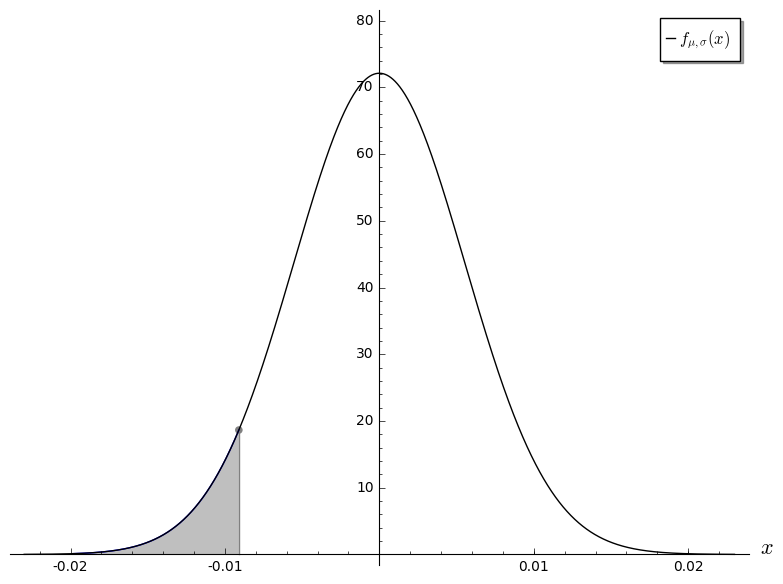
\includegraphics[scale=0.5]{chart1.png}
\end{center}
\caption{Rozkład względnych zmian cen złota z zacienionym poziomem tolerancji} \label{czynnosci_GD}
\end{figure} 


Oznaczmy teraz $k$ - kwantyl rzędu $\alpha$ dla standardowego rozkładu normalnego, czyli bardziej formalnie 
$$k=\Phi_{\mu=0,\sigma^{2}=1}^{-1}(\alpha)=\sqrt{2} erf^{-1}(2\alpha-1).$$
Możemy więc zastosować przekształcenie
$$VaR_{\alpha}^{rel}   =\sigma \sqrt{2} erf^{-1}(2\alpha-1)=\sigma \cdot k$$
z którego wynika że $VaR_{\alpha}^{rel}$ wyliczyć można korzystając z tablic kwantyli standardowego rozkładu normalnego. Dla $\alpha=0.05$ mamy $k=-1.645$. Odchylenie standardowe $\sigma=0.005532$. Zatem
$$VaR_{\alpha}^{rel}=\sigma \cdot k= 0.005532 \cdot (-1.645)=-0.0091$$

Bezwzględną wartość narażoną na ryzyko obliczamy korzystając ze wzoru
$$VaR = V \cdot |VaR^{rel}|.$$
Jeśli ustalimy $V=10000\$$ to otrzymamy $VaR = 10000\$ \cdot |-0.0091| = 91\$ $.

Rozważmy teraz przypadek gdy w portfelu inwestycyjnym znajduje się więcej niż jedna pozycja. Weźmy portfel $n$-instrumentowy. Niech
$$V=\begin{bmatrix}
 v_1 \\ 
 v_2 \\
\vdots \\
v_n
\end{bmatrix}$$
będzie wektorem wartości kolejnych instrumentów w portfelu.

Założyliśmy wcześniej, że rozkład zmian cen każdego instrumentu w portfelu jest rozkładem normalnym. Ponadto zmiany te są wzajemnie ze sobą skorelowane. Zmiana wartości całego portfela jest kombinacją liniową zmian wartości poszczególny instrumentów, mamy więc do czynienia z wielowymiarowym rozkładem normalnym. Wielowymiarowy rozkład normalny zadany jest wektorem wartości średnich rozkładów $\mu$ oraz kwadratową macierzą kowariancji $\Sigma$
$$\mu=\begin{bmatrix}
 \mu_1 \\ 
 \mu_2 \\
\vdots \\
\mu_n
\end{bmatrix},\Sigma=\begin{bmatrix}
\sigma_{11} & \sigma_{12} & \hdots & \sigma_{1n} \\ 
\sigma_{21} & \sigma_{22} & \hdots & \sigma_{2n} \\
\vdots & \vdots & \ddots & \vdots\\
\sigma_{n1} & \sigma_{n2} & \hdots & \sigma_{nn}
\end{bmatrix}. $$

Ze względu na początkowe założenia wektor $\mu$ będzie tutaj wektorem zerowym. Korzystając z własności wielowymiarowego rozkładu normalnego możemy obliczyć wariancję rozkładu zmian wartości całego portfela 


$$ \sigma_{Portfela}^2 = V^T  \cdot \Sigma \cdot V =  \begin{bmatrix}
 v_1 & v_2 & \hdots & v_n
\end{bmatrix} 
\cdot
\begin{bmatrix}
\sigma_{11} & \sigma_{12} & \hdots & \sigma_{1n} \\ 
\sigma_{21} & \sigma_{22} & \hdots & \sigma_{2n} \\
\vdots & \vdots & \ddots & \vdots\\
\sigma_{n1} & \sigma_{n2} & \hdots & \sigma_{nn}
\end{bmatrix}  
\cdot
\begin{bmatrix}
 v_1 \\ 
 v_2 \\
\vdots \\
v_n
\end{bmatrix}
=\sum_{i=1}^{n}\sum_{j=1}^{n}w_i w_j \sigma_{ij}.
$$


Mając wyznaczoną wariancję zmian wartości całego portfela, traktujemy ten rozkład jako jednowymiarowy. Można zatem wyznaczyć $VaR^{rel}$
$$VaR^{rel}=\sigma_{Portfela} \cdot k,$$
a także bezwzględną $VaR$
$$VaR = (\sum_{i=1}^{n}v_i) \cdot VaR^{rel}.$$.



\subsection{Metoda symulacji historycznej}



Metoda symulacji historycznej nie zakłada normalności rozkładu zmian cen, w ogóle nie są podejmowane jakiekolwiek wstępne założenia co do tego rozkładu. Rozkład ten opiera się wyłącznie na danych historycznych. Algorytm jako dane wejściowe przyjmuje względne zmiany cen aktywów, tworzy szereg wartości portfela. Mając szereg wartości portfela tworzymy szereg różnic pomiędzy wartością portfela każdego dnia a początkową wartością portfela. Szereg ten sortujemy rosnąco. Z tego szeregu wyznaczając odpowiedni (na podstawie założonego poziomu ufności) kwantyl otrzymujemy $VaR$.\\









 











\newpage
\section{System Akka}


\section{Projekt aplikacji}


\newpage














%%%%%%%%%%%%%%%%%%%%
%%%%%%%%%%%%%%%%%%%
%%%%%%%%%%%%%%%55









































































































































\section{Old Wstęp}      %* oznacza, że ta sekcja nie będzie numerowana   



Celem realizowanej pracy inżynierskiej będzie zaprojektowanie i zaimplementowanie klastra obliczeniowego w systemie Akka, który będzie wyliczał Value at Risk metodą symulacji Monte Carlo. 
\\
\\
Dla zadanego portfela składającego się z instrumentów finansowych, którego wartość oznaczymy zmienną losową $X$, pewnego przedziału czasowego $t$ oraz poziomu ufności $\alpha$, $VaR$ definiujemy jako maksymalną stratę wartości portfela jaką możemy ponieść w czasie $t$ zakładając poziom ufności równy $\alpha$.
\\
Załóżmy, że przedział czasowy $t$ jest stały. Wówczas $VaR$ można sformalizować jako
$$VaR_{\alpha}=inf\{ x\in \mathbb{R}:P(X+x<0) <  1-\alpha \}$$
\\
\\
Dla zobrazowania idei, przyjmijmy dla przykładu, że mamy portfel o wartości początkowej $1.000.000 USD$. Niech przedział czasowy $t=24h$ , poziom ufności $\alpha=0,95$. 
\\
Niech $VaR_{\alpha}$ będzie równe $70.000 USD$. Oznacza to, że w ustalonym przedziale $24h$ prawdopodobieństwo straty na portfelu przekraczające $70.000 USD$ jest równe $0,05$.  
\\
\\
\noindent Istnieją trzy główne metody obliczania VaR:

\begin{itemize}
  \item metoda kowariancji,
	\item metoda symulacji historycznej,
	\item metoda symulacji Monte Carlo.

\end{itemize}
Właśnie ta ostatnia wymaga największego nakładu mocy obliczeniowej. Rozproszenie obliczeń w klastrze może okazać się strategią znacznie przyśpieszającą wykonanie symulacji. 
\\
\\
Omówmy najpierw powyższe trzy metody wyznaczania VaR. 


\subsection{Metoda kowariancji}

Metoda kowariancji jest najprostsza i najszybsza do wykonania. Zakłada ona bowiem że rozkład zmian cen każdego aktywa w portfelu jest rozkładem normalnym. Założenie to nie jest prawdziwe, choć dla instrumentów bazowych takich jak akcje czy obligacje jest to całkiem dobre przybliżenie. Musimy zacząć od obliczenia $VaR$ każdej pozycji w portfelu. $VaR$ dla pojedynczej pozycji obliczamy wg. wzoru:

$$ VaR = k \cdot \sigma \cdot P $$

\noindent Gdzie:\\
\noindent $ k $ - pole pod wykresem gęstości prawdopodobieństwa dla założonego poziomu ufności, 
$ \sigma $ to zmienność czyli odchylenie standardowe rozkładu zmian cen, a $ P $ to wartość danej pozycji.
Aby policzyć VaR całego portfela po korzystamy ze wzoru:
$$ VaR=\sqrt{V \times C \times V^{T}} $$
\noindent Gdzie:\\
\noindent $ V $ - wektor wierszowy wartości $VaR$ dla każdej indywidualnej pozycji, $ C $ - kwadratowa macierz korelacji cen między instrumentami finansowymi, $ V^{T} $ - transponowana macierz V.\\

\subsection{Metoda symulacji historycznej}
Metoda symulacji historycznej nie zakłada normalności rozkładu zmian cen. Rozkład ten opiera na danych historycznych. Jako dane wejściowe przyjmuje względne zmiany cen aktywów, tworzy szereg wartości portfela. Mając szereg wartości portfela tworzymy szereg różnic pomiędzy wartością portfela każdego dnia a początkową wartością portfela. Szereg ten sortujemy rosnąco. Z tego szeregu wyznaczając odpowiedni (na podstawie założonego poziomu ufności) percentyl otrzymujemy $VaR$.\\








\newpage

\subsection{Metoda symulacji Monte Carlo}


Od metody symulacji historycznej  metoda symulacji Monte Carlo różni się tym, że nie posiadamy szeregów zmian cen. Generujemy je za pomocą generatora liczb pseudolosowych.
\\
\\
Zakładamy normalność rozkładu cen każdego z instrumentów w portfelu (choć jest to prawda jedynie w przybliżeniu).  Implikuje to fakt, że rozkład wartości całego portfela również będzie normalny (wartość portfela jest kombinacją liniową wartości poszczególnych instrumentów).
\\
\\
Dla jednego instrumentu w portfelu zadanie jest proste, ponieważ wygenerowanie szeregu względnych zmian cen polega na wylosowaniu liczb z RN o parametrach
$$\mu =0, \sigma =1 $$
\\
Oraz wymnożenie każdego elementu szeregu przez zmienność tego instrumentu. Na podstawie tych wartości początkowej portfela oraz wygenerowanych zmian względnych tworzymy szereg wartości portfela. Szereg sortujemy i na podstawie współczynnika ufności $\alpha$ wyznaczamy percentyl który jest szukaną VaR.
\\
\\
W przypadku gdy w portfelu jest więcej niż 1 instrument sytuacja się komplikuje, ponieważ musimy wziąć pod uwagę korelacje pomiędzy zmianami cen poszczególnych instrumentów.  Informacje o korelacjach można przechowywać w macierzy korelacji lub macierzy kowariancji. Algorytm używa macierzy kowariancji gdyż posiada ona dodatkowo informacje o wariancji każdej zmiennej.
\\
Niech
$$
\sum =\begin{bmatrix}
\sigma_{11} & \cdots  & \sigma_{1n}\\ 
 \vdots & \ddots  & \vdots \\ 
 \sigma_{n1}& \cdots  & \sigma_{nn}
\end{bmatrix}
$$
\\
Wtedy wartość $ \sigma_{kk} $ ( na przekątnej macierzy) jest wariancją zmiennej $ X_{k} $.
Zaś $ \sigma_{ij} $ gdzie $ i \neq j $, jest kowariancją zmiennych $ X_i $,  $ X_j $.
\\
\\
Algorytm zaczynamy od wygenerowania dla każdego instrumentu szeregu liczb pseudolosowych z rozkładu normalnego, znormalizowanego.  
\\
Niech 
\begin{itemize}
  \item $  X $ - wektor składający się z elementów pojedynczego szeregu zmian cen bez uwzględnienia korelacji
	\item $ Y $ - wektor składający się z elementów pojedynczego szeregu zmian cen po uwzględnieniu korelacji
	\item $ C  $ - macierz spełniająca następujące równanie $ C  C^{T} = \Sigma $
	\item $  \mu $ - ustalona średnia rozkładu zmian cen, w większości przypadków będzie to 0 (przy krótkich okresach symulacji wartość oczekiwana współczynnika zwrotu z inwestycji jest bliska zeru).

\end{itemize}
Wyznaczenie wektor $Y$ sprowadza się do rozwiązania równania
$$Y = \mu + CX = CX $$
Należy zatem zacząć od znalezienia macierzy $C$. Jednym z efektywnych numerycznie algorytmów rozwiązania równania
$$\Sigma = CC^T $$
jest diagonalizacja macierzy $\Sigma$ i skorzystanie z własności macierzy diagonalnej 

$$ \Sigma =  P \Delta P^T = P \Delta^{\frac{1}{2}} \Delta^{\frac{1}{2}}P^T=P \Delta^{\frac{1}{2}} (\Delta^{\frac{1}{2}})^T P^T=P \Delta^{\frac{1}{2}} (P \Delta^{\frac{1}{2}})^T=CC^T $$\\

Wyznaczenie $P$ oraz $\Delta$ może odbyć się przed właściwym rozproszeniem algorytmu ponieważ jest to stosunkowo szybkie obliczenie (w porównaniu z samą symulacją).\\
\\
Teraz możemy jasno uzasadnić sposób działania samej symulacji. Oznaczmy 
$$ P=\begin{bmatrix} P_1 & \vdots & P_2 & \vdots  & \hdots & \vdots & P_n \end{bmatrix} $$
gdzie $P_i$ to wektor własny macierzy kowariancji dla instrumentu $i$. Zaś z własności macierzy diagonalnej $\Delta$ zachodzi własność
$$\Delta^{\frac{1}{2}}=\begin{bmatrix} \sqrt{\Delta_1} &  \cdots &0 \\  \vdots & \ddots  & \vdots \\ 0& \cdots & \sqrt{\Delta_n} \end{bmatrix}$$\\
\\
gdzie $\sqrt{\Delta_i}$ jest $i$-tą wartością własną macierzy kowariancji.\\
Mamy zatem 
$$Y = CX = P \Delta ^ {\frac{1}{2}} X$$
Niech $y_i$ będzie $i$-tym elementem wektor $Y$. Liczbę instrumentów w portfelu oznaczmy $N$. Załóżmy, że obliczenia wykonujemy dla instrumentu z indeksem $k$.\\
Wtedy przez $P_i[k]$ rozumiemy $k$-ty element wektora własnego dla instrumentu $i$. Mamy
$$y_i=\sum_{i=1}^{N}(P_i[k]\cdot\sqrt{\Delta_i}\cdot x_i)$$.\\
\\
Zaletą tego podejścia jest fakt, że każdy element wektora $Y$ można wyznaczyć niezależnie od pozostałych. Z punktu widzenia przetwarzania w klastrze jest to istotne, ponieważ każdy węzeł będzie mógł przeprowadzać wyznaczanie elementów tego wektora niezależnie, nie oczekując na pozostałe węzły.\\
\\
Warto wspomnieć dlaczego właśnie system Akka będzie odpowiednim narzędziem do stworzenia takiego klastra. Akka, napisana w języku Scala opiera się na modelu aktorów stworzonym do obliczeń współbieżnych i rozproszonych. Aktorzy są podstawowymi jednostkami modelu aktorów. Ze względów bezpieczeństwa aktorzy nie komunikują się w inny sposób jak poprzez wysyłanie wiadomości. Po odebraniu wiadomości aktor może:

\begin{itemize}
  \item stworzyć skończoną liczbę nowych aktorów,
	\item wysłać skończoną liczbę wiadomości do innych aktorów,
	\item zdeterminować swoje zachowanie gdy nadejdzie następna wiadomość.

\end{itemize}
Tylko te trzy możliwości wydają się być ograniczające, jednak ta prostota zapewnia bezpieczeństwo i łatwość tworzenia aplikacji. \\
\\
Dodatkowo Akka jest wysoce zoptymalizowana zarówno jeśli chodzi o przesyłanie wiadomości pomiędzy aktorami (do 50 mln. wiadomości / sekundę na pojedynczej maszynie), jak i oszczędność pamięci (1 GB pamięci pomieści 2,5 mln. aktorów). \\
\\
Dzięki hierarchiczności aktorów i ich specjalnym typie Supervisor (kierownik) lokalne i rozproszone węzły mogą leczyć się same (Aktorzy podrzędni są leczeni przez aktorów nadrzędnych). Dzięki temu rozproszone systemy są odporne na uszkodzenia węzłów. \\
\\
Nie należy zapominać o fakcie że język Akka powstał na platformie JVM, bogatej w biblioteki i narzędzia (które można wykorzystać w Scali pomimo że same zostały napisane w innym języku platformy JVM).\\

\newpage
\section{Old Analiza problemu}



\subsection{Istotność wyliczania miar ryzyka}
Value at Risk jest standardową już miarą ryzyka stosowaną prawdopodobnie przez znaczącą większość instytucji finansowych na poziomie ufności co najmniej 95\% . Bazylejski Komitet Nadzoru Bankowego stosuje poziom ufności 99\%. Zaimplementowanie VaR we wczesnych latach '90 przez JP Morgan i upublicznienie tej technologii, pomogło przyśpieszyć wyjście z kryzysu finansowego rozpoczętego w roku 1987.\\
\\


Pomijając zaufanie bankierów do tej metody trzeba wspomnieć o jej istotnej przewadze nad wskaźnikami VBPM: VaR jest w stanie określić prawdopodobieństwo straty na portfelu, większej niż ustalona wcześniej kwota. \\
\\

Również bardzo ważną zaletą VaR jest to, VaR zależy od wzajemnych korelacji zmian cen w portfelu. Pomaga to inwestorom i instytucjom finansowym zdywersyfikować portfel w odpowiedni sposób.


\subsection{Ograniczone dane a szybkość i dokładność obliczeń}
Symulacja Monte Carlo, zamiast metody historycznej, używana jest gdy nie mamy dostępu do wystarczająco długich i dokładnych informacji o zmianach cen instrumentów w portfelu. Symulacja historyczna jest szybsza, ponieważ nie musimy generować liczb pseudolosowych ani też stosować względnie kosztownego obliczeniowego wzoru na Skorelowane Zmiany Cen (musimy tego wzoru użyć setki tysięcy, lub nawet miliony razy, w zależności od liczby symulacji Monte Carlo). \\
\\
Po drugie symulacja historyczna jest dokładniejsza, bo korzysta z historycznych (a zatem rzeczywistych) rozkładów zmian cen, a nie z rozkładu normalnego. Mimo to przy odpowiedniej liczbie symulacji, metoda Monte Carlo daje bardzo dokładne wyniki (zbliżone do wyników symulacji historycznej).

\newpage

\section{Old Projekt systemu}


\subsection{System jako eksperyment badający przyśpieszenie obliczeń}

Projekt ten jest tworzony w celach eksperymentalnych, nie komercyjnych. Eksperyment ten ma pokazać, czy rzeczywiście system rozproszony oparty na Modelu Aktorów będzie szybszy od systemu sekwencyjnego, i jeśli tak – to w jakim stopniu. Na wejściu będzie można załadować dowolny portfel aktywów - Kluczowy wpływ na szybkość będzie tu mieć ilość pozycji w portfelu. Cały system opiera się na węzłach - Aktorach. Będą nas interesować dwa typy węzłów - Aktor-Master oraz Aktor-Dziecko. Aktor Master stworzy pewną (również sterowalną przez argument podany do programu) liczba Aktorów-Dzieci, którzy wykonują dla niego pewne obliczenia, a które On potem podaje ostatecznemu przetwarzaniu w celu obliczenia VaR. Chcemy pokazać, że czas obliczenia VaR, jest zależny od liczby Aktorów, w jaki sposób. Aktorzy mogą wykonywać się również na jednej maszynie - uzyskamy przyśpieszenie jedynie wtedy gdy liczba rdzeni procesora będzie większa niż 1.\\
\\
Jednak Aktorzy mogą wykonywać się również zdalnie, na różnych maszynach, warunkiem jest aby były połączone przez sieć, w tym przypadku tym przypadku tzw. protokół Akka-Remoting. (działający domyślnie na serwerze Netty, w warstwie transportowej operuje na protokole TCP, na portach >2500).



\subsection{Opisy protokołów}

Program działa na serwerze Netty. Używa protokołu tcp. Każdy aktor posiada adres w systemie który nie jest zależny od maszyny na której się wykonuje. 
\\
W moim przypadku do eksperymentów użyłem 2 komputerów, oto ich specyfikacje:
\begin{itemize}
  \item Fujitsu AH531 (CPU to 2-rdzeniowy Intel Celeron taktowany zegarem 1,5 GHz
	\item Lenovo Thinkpad  T510 (CPU - 4-rdzeniowy Intel Core i5

\end{itemize}

Próbowałem dwóch różnych systemów komunikacji. Jeden połączenie przez router 801.11b (max transfer 11Mb/s).
\\
Drugi to bezpośrednie połączenie kable Gigabit Ethernet dwóch komputerów. Przepustowość - 1Gb/s
\\

\subsection{Opisy algorytmów}

Opisy algorytmów zacznijmy od przypomnienia faktu, że jest to symulacja Monte Carlo, więc wiąże się to z wygenerowaniem dużej (ok. 100000) ilości liczb pseudolosowych dla każdej pozycji w portfelu ( będą to liczby zmiennoprzecinkowe podwójnej precyzji, tzw. typ double). Dodatkowo te długie szeregi liczb będą generowane nie w rozkładzie jednostajnym, lecz normalnym, konkretnie o parametrach $ N (0,1) $ . Na szczęście wbudowana w Javę klasa Double, posiada metodę do wyznaczania liczb pseudolosowych o takim rozkładzie.
\\
\\
Aby przyśpieszyć obliczenia, algorytm symulacji będzie rozproszony. Aktorzy-Dzieci (najniższe hierarchią węzły sieci) generować będą części Szeregów Normalnych. Warunkiem koniecznym jest, aby Aktorzy-Dzieci dla każdej pozycji w portfelu generowali Szeregi Normalne o tych, samych indeksach, będzie to konieczne do wyliczenia Skorelowanych Zmian Cen.
\\
Oto wzór na i-ty element szeregu Skorelowanych Zmian Cen dla instrumentu k:

$$y_i=\sum_{i=1}^{N}(P_i[k]\cdot\sqrt{\Delta_i}\cdot x_i)$$.\\

Gdzie:
\begin{itemize}
  \item $N$ - liczba instrumentów w portfelu,
	\item $y_i$ - $i$-ty element szeregu Skorelowanych Zmian Cen,
	\item $P_i[k]$ - $k$-ty element wektora włanego dla instrumentu $i$,
	\item $\sqrt{\Delta_i}$ - $i$-ta wartość własna macierzy kowariancji,
	\item $x_i$ - $i$-ty element szeregu liczb z rozkładu normalnego.

\end{itemize}


Jak widać elementów szeregów Skorelowanych Zmian Cen będzie dokładnie tyle samo co elementów Szeregów Normalnych. Aktorzy-Dzieci Po otrzymaniu odpowiednich "porcji" Szeregów Normalnych liczą dla nich Skorelowane Zmiany Cen. Po tej Operacji posiadają Skorelowane Zmiany Cen dla każdego instrumentu w portfelu. Mogą więc wyliczyć szeregi Zmian Bezwzględnych, używając pierwotnych wartości pozycji z obiektu Wallet. Zmiany Bezwzględne następnie sumują i korzystając z wbudowanego w Javę sortowania przez scalanie (nie korzystam z własnej implementacji gdyż okazała się wolniejsza), sortuję porcję zsumowanych Zmian Bezwzględnych. Przesyłane są one następnie do Aktor-Mastera (nadrzędnego), który scala je i sortuje tym samym algorytmem który wykorzystały Aktorzy-Dzieci. \\
\\
Warto wyjaśnić dlaczego sortowanie przez scalanie jest tutaj najbardziej odpowiednim algorytmem sortującym. Po pierwsze jak wiadomo nawet w najgorszym przypadku ten algorytm posiada złożoność asymptotyczną $ O (n \cdot log(n)) $ ( np. Quick Sort, choć szybki w przeciętnym przypadku nie posiada tej własności). Po drugie Aktor-Master ostatecznie otrzymuje szeregu zsumowanych Zmian Bezwzględnych w porcjach, zatem i tak musiałby je jakoś scalić, a sortowanie przez scalanie wykonuje to jako część algorytmu.\\
\\
Mając już pełny posortowany szereg zsumowanych Zmian Bezwzględnych, musimy wyznaczyć odpowiedni percentyl, na podstawie wcześniej ustalonego poziomu ufności. Ten percentyl to szukana Wartość Narażona na Ryzyko.



\subsection{Omówienie hierarchii węzłów sieci}

Na potrzeby analizy algorytmu wystarczy wiedza, że nasz Aktor-Master stoi stopień wyżej w hierarchii od Aktorów-Dzieci. Jednak warto nadmienić, że ponad naszym Aktorem-Masterem stoi systemowy Guardian-System-Aktor (zwany też w niektórych źródłach rootem), który jest rodzicem Aktora-Mastera, i który działa poprawnie nawet gdy wszyscy Aktorzy niższe w hierarchii ulegną awarii. Ma więc on możliwość naprawy systemu Aktorów, tak jak każdy Aktor w systemie Akka posiadający aktorów niżej w hierarchii ma możliwość ich naprawy (jest to jedno głównych założeń systemu Akka). \\
\\
Warto tutaj powiedzieć że ilość hierarchii w omawianym systemie nie powinna być większa - a raczej, konkretnie mówiąc stworzenie większej ilości hierarchii spowoduje więcej problemów niż korzyści. Przy założeniu takiej samej liczby Aktorów, a większej liczby hierarchii Aktorzy będą mieli więcej danych do rozsyłania, co wiąże się z dłuższym działaniem programu.


\subsection{Omówienie wiadomości przesyłanych między węzłami sieci}

Zacznijmy omówienie tej kwestii od samego początku wykonywania się programu. Czyli - na początku, w funkcji main(), wczytywany jest i parsowany plik wallet.xml, który przez klasę WalletParser konwertowany jest do klasy Wallet. Klasa Wallet zawiera wszystkie potrzebne informacje o pozycjach znajdujących się w portfelu, czyli:
\begin{itemize}
  \item numer identyfikacyjny pozycji,
	\item nazwa pozycji (np. gold, oil) ,
	\item wartość początkową pozycji w portfelu (wyrażoną domyślnie w USD),
	\item dzienna zmienność cenowa pozycji,
	\item wartość własną pozycji w macierzy korelacji cen,
	\item wektor własny pozycji w macierzy korelacji cen.

\end{itemize}

Następnie Tworzymy Guardian-System-Actora, który uruchamia Aktora-Mastera. Wysyłamy Masterowi  obiekt typu Wallet, oraz Integer oznaczający liczbę dzieci którą ma uruchomić. Po otrzymaniu tych wiadomości Master uruchamia dzieci i rozdziela ilość pracy ( czyli ilość Szeregów Normalnych do wygenerowania) pomiędzy swoich Aktorów-Dzieci, starając się dzielić zadania między Dzieci możliwie jak najbardziej równomiernie. Ze względu na fakt, że liczba symulacji nie musi być podzielna przez liczbę Dzieci, nie zawsze będzie możliwy idealnie równomierny podział, jednak problem ten nie jest aż tak bardzo istotny. \\
\\
Obiekt Wallet jest następnie sklonowany ( użycie do wysłania tej samej referencji na jednej maszynie spowoduje, że Aktorzy dzieci będą przetwarzać ten sam obiekt, co jest niedopuszczalne) tyle razy, ile mamy dzieci ( musi być to tzw. kopia głęboka, ze względu na zagnieżdżone struktury danych). Wallet nie implementuje interfejsu Cloneable, a własnoręcznie napisane implementacje metod kopiujących obiekty nie zazwyczaj nie działają poprawnie, zdecydowałem się użyć zewnętrznej biblioteki Cloning wydanej na licencji Apache 2.0. Sklonowane obiekty typu Wallet wysyłane są do Dzieci, wysyłany jest też Integer oznaczający ile liczb o rozkładzie normalnym dziecko ma wygenerować. Po całym przetwarzaniu opisanym w sekcji Opisy Algorytmów, Aktorzy-Dzieci Wysyłają do Mastera posortowane fragmenty Szeregów Cen Bezwzględnych. W tym miejscu kończy się przesyłanie danych między węzłami sieci, pozostaje tylko praca do wykonania przez Mastera.








\section{Old Implementacja sytemu}

\subsection{Użyte technologie}

Wersja JVM wykorzystana w projekcie to JVM 8, wersja języka Scala to 2.11.7. \\
\\
Framework Akka, pozwalający na korzystanie z systemu Aktorów, i klas umożliwiających zdalną komunikację węzłów, jest w wersji 2.4.0.\\
\\
Dodatkowo używam biblioteki Cloning, umożliwiającej tworzenie głębokich kopii obiektów nawet jeśli nie implementują interfejsu Cloneable. Ta biblioteka jest wersji 1.9.2.





\newpage
\bibliographystyle{plain}

\bibliography{P2P}
Philip Best, Wartość narażona na ryzyko, tłum. Andrzej Komański,
\\
Kraków 2000 ISBN: 82-88597-01-9.

\end{document}
